% !TEX root = ../../main.tex

\chapter{GASP: Generalized Agglomerative Algorithm for Signed Graph Partitioning}\label{chapter:GASP}

In this chapter, we propose a theoretical framework that generalizes simple and fast algorithms for hierarchical agglomerative clustering to weighted graphs with both attractive and repulsive interactions between the nodes. This framework defines GASP, a Generalized Algorithm for Signed graph Partitioning, and allows us to explore many combinations of different linkage criteria and cannot-link constraints. 
We prove the equivalence of existing clustering methods to some of those combinations and introduce new algorithms for combinations that have not been studied before. 
We study both theoretical and empirical properties of these combinations and prove that some of these define an ultrametric on the graph.
We conduct a systematic comparison of various instantiations of GASP on a large variety of both synthetic and existing signed clustering problems, in terms of accuracy but also efficiency and robustness to noise. 
Lastly, we show that some of the algorithms included in our framework, when combined with the predictions from a CNN model, result in a simple bottom-up instance segmentation pipeline.
Going all the way from pixels to final segments with a simple procedure, we achieve state-of-the-art accuracy on the CREMI 2016 EM segmentation benchmark without requiring domain-specific superpixels.


\begin{figure*}[t]
\centering
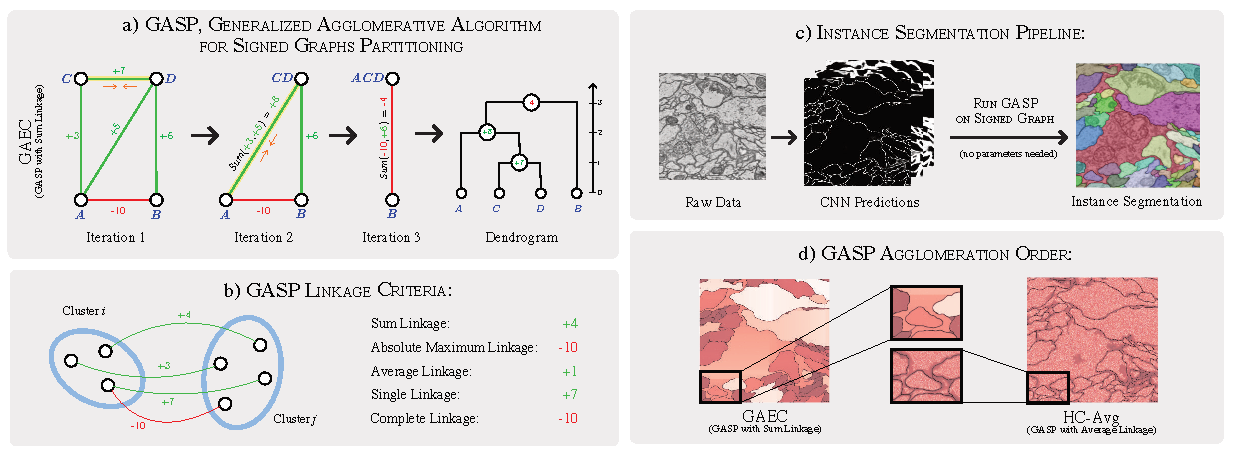
\includegraphics[width=\textwidth]{figures/GASP/intro_image_v6.pdf} % left bottom right top
\caption{\textbf{(a)} Some iterations of \algname{} on a graph with attractive (green) and repulsive (red) interactions. At each iteration, the yellow edge with highest weight is contracted (example with sum linkage criterion is shown). \textbf{(b)} Linkage criteria demonstrated on two small clusters (see definitions in Table~\ref{tab:linkage-criteria} below).  \textbf{(c)} Application of \algname{} to instance segmentation: we show raw data from the CREMI neuron-segmentation challenge and some predictions of our CNN model, where white pixels represent boundary evidence. \textbf{(d)} 
Seemingly similar linkage criteria can result in very different clustering dynamics, as shown in this example: color coded sequence of merges from early (white) via late (brown) to never (black).
% \algname{} agglomeration order for sum and average linkage: we show which pairs of neighboring pixels were merged first (white), later on (brown/red), or never (black).
\label{fig:intro_figure}}
\end{figure*}


\renewcommand\theadfont{\scriptsize}
\begin{table*}[t]
    \centering
    \scriptsize
    \begin{subtable}[t!]{\textwidth}\centering
        \begin{tabular}{c |c  c  c  c  c}
        \multicolumn{1}{c|}{\multirow{2}{*}[-1.5em]{{\Large GASP}}} 
        & \thead{Sum\\Linkage} & \thead{Absolute Maximum\\Linkage} & \thead{Average\\Linkage} & \thead{Single\\Linkage} & \thead{Complete\\Linkage} \\
 % \multicolumn{1}{c}{} 
 & $\displaystyle \sum_{e\in E_{ij}} \cost_e$  & $\displaystyle \cost_e$ with $\displaystyle e = \argmax_{t\in E_{ij}} |\cost_t|$ & $\displaystyle \sum_{e\in E_{ij}} \cost_e \bigg/ \big|E_{ij}\big| $ &  $\displaystyle \max_{e\in E_{ij}} \cost_e$ & $\displaystyle \min_{e\in E_{ij}} \cost_e$ \\ \midrule
 % \cmidrule{2-6}

            \thead[c]{Unsigned graphs} & \thead{-} &\tikzmark{a} \thead{\textbf{HC-Single}} &\tikzmark{g} \thead{\textbf{HC-Avg}} &\thead{\textbf{HC-Single}}\tikzmark{z} &\thead{\textbf{HC-Complete}} \tikzmark{b} \\
            \thead[c]{Signed graphs} & \thead{GAEC \cite{keuper2015efficient}} &  \thead{\textbf{Mutex Watershed} \cite{wolf2018mutex}}& \tikzmark{f} \thead{\textbf{HC-Avg}} &\thead{\textbf{HC-Single}} \tikzmark{e} &\thead{\textbf{HC-Complete}}\tikzmark{w} \\
            \thead[c]{Signed graphs + \\cannot-link-constr} & \thead{\colorbox{yellow}{HCC-Sum}} % \thead{Greedy Fixation \cite{levinkov2017comparative}} 
            & \thead{\textbf{Mutex Watershed} \cite{wolf2018mutex}}& \thead{\colorbox{yellow}{HCC-Avg}} &  \thead{\colorbox{yellow}{HCC-Single}} \tikzmark{d} &   \thead{\textbf{HC-Complete}} \tikzmark{c} \\
            % \multicolumn{2}{c|}{\multirow{2}{*}[-0.5em]{\thead{\textbf{\algname{} linkage criteria} $\,\,\interact(S_u ,S_v)$}}}  & \multirow{2}{*}[-0.5em]{\thead{\textbf{Unsigned Graphs}}} & \multicolumn{2}{c}{\thead{\textbf{Signed Graphs}}}  \\        
            % \multicolumn{2}{c|}{} &  &  \multicolumn{1}{c}{\thead{No Constraints}} & \thead{With Constraints} \\ \midrule
             

            %  Sum: & $\displaystyle \sum_{e\in E_{uv}} \cost_e$ & \thead{Sum Linkage\\Hier. Aggl. Clust.} & \thead{GAEC \cite{keuper2015efficient}} & \thead{Greedy\\Fixation \cite{levinkov2017comparative}} \\ 
            
             


            %  \makecell[r]{Abs. Max:} & 
            % $\displaystyle \cost_e$ with $\displaystyle e = \argmax_{t\in E_{uv}} |\cost_t|$
            %    & \thead{Single Linkage\\Hier. Aggl. Clust.} & \thead{Mutex\\Watershed \cite{wolf2018mutex}} & \thead{Mutex\\Watershed \cite{wolf2018mutex}} \\
             


            %  \makecell[r]{Average:} & $\displaystyle \sum_{e\in E_{uv}} \cost_e \bigg/ \big|E_{uv}\big|  $ & \thead{ Average Linkage\\ Hier. Aggl. Clust.} & \thead{\textbf{NEW}} & \thead{\textbf{NEW}}\\ 

            % Max: & $\displaystyle \max_{e\in E_{uv}} \cost_e$ & \thead{Single Linkage\\Hier. Aggl. Clust.} & \thead{\textbf{NEW}} & \thead{\textbf{NEW}}\\ 

            % Min:& $\displaystyle \min_{e\in E_{uv}} \cost_e$ & \thead{Complete Linkage\\ Hier. Aggl. Clust.}  & \thead{\textbf{NEW}} & \thead{\textbf{NEW}}

        \end{tabular}
    \end{subtable} 
    \caption{Conceptual contribution: Properties of clustering algorithms included in the proposed \algname{} framework, given a linkage criterion, a type of graph (signed or unsigned) and the optional use of cannot-link constraints. New constrained hierarchical clustering algorithms (HCC) proposed in this thesis are highlighted in yellow. For algorithms typeset in bold font we prove that they define an ultrametric on the graph (Eq.~\ref{eq:UM_def}). For algorithms in the green box we show that they are weight-shift invariant (Prop.~\ref{prop:weight_shift_invariant}). 
    Notation: 
    % given a signed graph $\mathcal{G}(V,E, w_e)$, we denote as 
    $E_{ij}=(S_i \times S_{j}) \cap E$ denotes the set of edges connecting two clusters $S_i, S_j \subseteq V$. } 
    \label{tab:linkage-criteria}
\end{table*}
\renewcommand\theadfont{\normalsize}


\section{Introduction}
In computer vision, the partitioning of weighted graphs has been successfully applied to tasks as diverse as image segmentation, object tracking and pose estimation. 
Most graph clustering methods work with positive edge weights only, which can be interpreted as similarities or distances between the nodes. These methods require users to specify the desired numbers of clusters (as in spectral clustering) or a termination criterion (e.g.\ in iterated normalized cuts) or even to add a seed for each object  (e.g.\ seeded watershed or random walker).  

Other graph clustering methods work with so-called \emph{signed graphs}, which feature both positive and negative edge weights corresponding to attraction and repulsion between nodes. The advantage of signed graphs over unsigned graphs is that balancing attraction and repulsion allows us to obtain a clustering without defining additional parameters. A canonical formulation of the signed graph partitioning problem is the \emph{multicut} or \emph{correlation clustering} problem \cite{kappes2011globally,chopra1991multiway}. This problem is NP-hard, though many approximate solvers have been proposed \cite{lange2018combinatorial,pape2017solving,beier2016efficient,yarkony2012fast} together with greedy agglomerative clustering algorithms \cite{keuper2015efficient,levinkov2017comparative,wolf2018mutex,kardoostsolving}. 
Agglomerative clustering algorithms for signed graphs have clear advantages: they are parameter-free and efficient. Despite the fact that a variety of these algorithms exist, no overarching study has so far been conducted to compare their robustness and efficiency or to provide guidelines for matching an algorithm to the partitioning problem at hand. 


The first contribution presented in this chapter is a simple theoretical framework that generalizes over agglomerative algorithms for signed graphs by linking them to hierarchical clustering (HC) on unsigned graphs (Section \ref{sec:algorithm}). This framework defines an underlying basic algorithm and allows us to explore its combinations with different linkage criteria and \emph{cannot-link constraints} (see Fig.~\hyperref[fig:intro_figure]{\ref*{fig:intro_figure}a}, \hyperref[fig:intro_figure]{\ref*{fig:intro_figure}b}, and Table~\ref{tab:linkage-criteria}). 
As second contribution, in Section \ref{sec:alg_update_rules}, we formally prove that some of the combinations correspond to existing clustering algorithms, and introduce new algorithms for combinations which have not been explored before. By analyzing their theoretical properties, we also show that some of them define an ultrametric on the graph (see Table~\ref{tab:linkage-criteria}).

Third, we evaluate the algorithms on a large variety of both existing and synthetically generated signed graph clustering problems (Section \ref{sec:neuro_segm_exp}). 
Fourth and finally, we also test the algorithms on \emph{instance segmentation} -- a computer vision task consisting of assigning each pixel of an image to an object instance -- by partitioning graphs whose edge weights are estimated by a CNN (see Fig.~\hyperref[fig:intro_figure]{\ref*{fig:intro_figure}c} and Section \ref{sec:experiments_discussion}).
Our experiments show that the choice of linkage criterion markedly influences how clusters are grown by the agglomerative algorithms (Fig.~\hyperref[fig:intro_figure]{\ref*{fig:intro_figure}d}), making some linkage methods more suited for certain types of clustering problems.
% We focus our comparison on three of the best-performing algorithms included in our framework, which are based on average, sum, and absolute maximum linkage criteria (see Table~\ref{tab:linkage-criteria}). We highlight their empirical properties by showing how clusters are grown differently depending on the algorithm.
We benchmark the clustering algorithms by focusing on their efficiency, robustness and tendency to over- or under-cluster. 
On instance segmentation, we show that the tested agglomerative algorithms strongly outperform recently proposed spectral clustering methods, and that average-linkage based agglomerative algorithms achieve state of the art results on the CREMI 2016 challenge for neuron segmentation of 3D electron microscopy image volumes of brain tissue. 

\begin{tikzpicture}[remember picture,overlay]
% (shift_along_horizontal, shift_along_vertical)
% a ---------------------------- b
%            g -----------------
%            f         e ------- 
%                      d         c
% 
\draw [green,line]($(a)+(0,2ex)$)--($(b)+(0.9ex,2ex)$)--($(c)+(0.9ex,-1.5ex)$) -- ($(d)+(1.4ex,-1.5ex)$) -- ($(e)+(1.4ex,-1.2ex)$) -- ($(f)+(-0.3ex,-1.2ex)$)--($(g)+(-0.3ex,-1.2ex)$)--($(a)+(0,-1.2ex)$)--cycle;
\end{tikzpicture}

% In Sec.~\ref{sec:spectral_clust}, we also show how \algname{} outperforms spectral clustering methods on the task of neuron segmentation and how on synthetic graphs it achieves similar scores to a recently proposed spectral method for signed graphs. 
% \TODO{Define HC abbrv}

% Our code is available at \url{https://github.com/abailoni/GASP}.






